\chapter{The Completion}
\label{ch:30}



\begin{center}
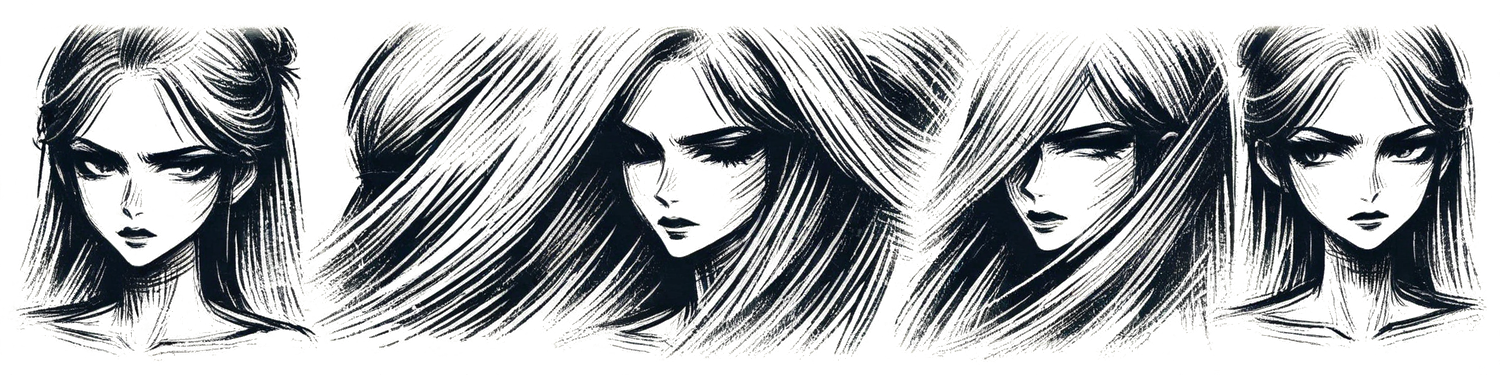
\includegraphics[width=\textwidth]{images/chapterImages/genesis_sketch_00131_.png}
\end{center}

The alert came at 2:47 AM. Sarah was already awake—sleep had become optional years ago, a luxury she occasionally indulged in for four-hour blocks. She saw the notification light up across seventeen different screens in the monitoring station simultaneously.

2019 KX₇. 1.2 kilometers across. Trajectory confirmed. Impact probability without intervention: 99.97\%.

Time to impact: 73 hours.

She felt nothing. No fear. No excitement. Just the immediate cascade of calculations, system checks, deployment sequences. The compulsion had evolved over twenty years from a driving force into something quieter, more integrated. Like breathing. Like heartbeat. Just what she did.

"Confirmation," she said into the comm. "I have eyes on the target."

Responses came from seventeen stations across the globe. Moscow. Cape Canaveral. Beijing. Mumbai. São Paulo. Everyone activated. Everyone working. The planetary defense network humanity had spent two decades building was about to be tested for the first time.

Not the first time, Sarah corrected herself. The first time this iteration of life had built it. Aurelia's version had existed 65 million years ago. Different technology. Same purpose. The pattern repeated.

"Grid status?" she asked.

"Eighty-three satellites operational," Marcus's voice came through. Still calm. Still measured. Twenty years since that night on the concrete floor and his voice still did something to her body. Still made her aware of herself in ways the compulsion couldn't quite override.

They'd been careful. Stayed professional. Worked together for six years, then requested separate assignments. Saw each other maybe twice a year at conferences. Brief conversations. Polite distance. The bruises had faded. The memory hadn't.

"Trajectory calculation complete," someone else said. Chen Wei, maybe. Or Park Min-jun. Hard to tell voices after this long. They all sounded the same when activated—focused, precise, emotionless.

Sarah pulled up the deflection model. The asteroid would pass within 47,000 kilometers of Earth's surface without intervention. Close enough to be visible to the naked eye. Close enough that every news network on the planet was already screaming about extinction.

They didn't know the grid existed. Not officially. The engineering had been done through thousands of private companies, disguised as commercial satellites, telecommunications infrastructure, weather monitoring. No single government controlled it. No one organization understood the full picture.

Except the activated. They all knew. Had built it collectively, each contributing their piece, none of them able to stop.

"Initiating sequence," Sarah said. "Gravitational anchors deploying in three... two... one... mark."

Eighty-three satellites shifted position simultaneously. Microscopic adjustments. Precise beyond human capability—or what human capability used to be. Each satellite generated a minuscule gravitational field. Individually meaningless. Together, enough to bend spacetime just slightly. Enough to alter the trajectory of 1.2 kilometers of rock moving at 30 kilometers per second.

"Field generation confirmed," Marcus said. "Deflection angle should be sufficient."

Should be. Twenty years of work. Trillions of dollars from budgets no one admitted existed. Relationships destroyed. Lives consumed. Maya's entire childhood sacrificed. David dead from exhaustion while coding the control systems. Thousands of marriages ended. Tens of thousands of people who couldn't explain to their families why they had to work, had to build, had to finish this thing they couldn't justify.

Should be.

The data came in over forty-eight hours. Sarah watched the asteroid's trajectory bend. Millimeter by millimeter. The curve changing. The impact probability dropping.

99.97\%.
94.23\%.
76.85\%.
43.12\%.
18.47\%.
2.35\%.
0.08\%.
0.00\%.

At 49 hours and 17 minutes after initial deployment, the asteroid's new trajectory was confirmed. It would miss Earth by 197,000 kilometers. Not even close. Barely worth noticing.

Humanity would survive. The planet would continue. Life would go on.

Sarah felt nothing.

\scenebreak

The celebration was held in Geneva. Neutral ground. The various agencies and organizations that officially didn't know about the grid suddenly had to acknowledge it existed. There were speeches. Awards. Recognition for people who'd sacrificed everything to build a system they couldn't explain.

Sarah wore a dress her ex-husband's new wife had helped Maya pick out. Black. Simple. Appropriate for someone who'd just saved the world and couldn't bring herself to care.

The ceremony was surreal. Dignitaries praising the engineering brilliance. Scientists marveling at the achievement. News anchors calling it humanity's greatest triumph. The definitive proof of human capability. Human choice. Human will.

None of them understood. They thought this was chosen. Thought the thousands of engineers and physicists and mathematicians had voluntarily dedicated decades to this project. Thought it was collaborative genius rather than synchronized programming.

Sarah stood in the reception hall with a glass of champagne she wasn't drinking and watched people celebrate. Marcus was somewhere on the other side of the room. She'd seen him during the ceremony—thinner than twenty years ago, grayer, the same intense focus in his eyes. He'd glanced at her once. Brief. Enough.

"Dr. Chen."

Sarah turned. A young woman, mid-twenties, too excited to be appropriate. "I just wanted to say thank you. I studied your genetic research in grad school. Your work on activation sequences changed everything."

Sarah's papers had been published twelve years ago. After too much pressure. After too many people activated and needed to understand what was happening to them. The revelation that human evolution was programmed had caused exactly the philosophical crisis James predicted. Religions fractured. Suicide rates spiked. A new wave of existential despair swept through the intellectual class.

Most people ignored it. Preferred to believe they were free. Preferred to think the genetic evidence was misinterpreted or overstated. Cognitive dissonance was powerful.

"You're activated," Sarah said, reading the young woman's body language. The intensity. The focus.

"Space propulsion capability," the woman said. "Started expressing two years ago. I'm working on fusion drive systems. Can't explain how I know it'll work, but I do. Just like you described."

"What's your name?"

"Dr. Yuki Tanaka. I've been trying to reach you for months. We're organizing. People with the new activation. There are thousands of us now. All working on the same thing—deep space travel. Interstellar capability. We think... we think there's another threshold coming."

Sarah had known. Had seen it in the genetic data years ago. The space travel capability was next. After planetary defense came expansion. After learning to protect the planet came learning to leave it.

The pattern unfolding. The program executing.

"When?" Sarah asked.

"Initial estimates say ten years. Maybe less. The compulsion is already strong. Stronger than the accounts from your generation described. We're going to build interstellar ships. We know we are. Can't stop even if we wanted to."

"Do you want to?"

Yuki considered this. "No. Maybe that's the programming. Maybe I'm supposed to want this. But it feels right. Feels like purpose. Feels like the most important thing I could possibly do with my existence."

Sarah thought of Aurelia. Standing with her dead mate. Then returning to work. The compulsion and the choice merged into something indistinguishable.

"Good luck," Sarah said.

"Will you help? We need expertise on the genetic mechanisms. On how the activation works. On—"

"No."

"But you're the foremost—"

"I'm done," Sarah said. "I did what I was programmed to do. The grid is built. The asteroid is deflected. My part is finished."

"But the space program—"

"Is yours. Not mine. I don't feel it. The compulsion for planetary defense is quiet now. Has been since we succeeded. Whatever's next is for your generation."

Yuki looked disappointed. Frustrated. She didn't understand yet that the compulsion was specific. Targeted. Once you fulfilled your function, it released you. Left you hollow and exhausted and trying to figure out what else there was.

"There's someone you should meet," Yuki said. "Another researcher. He's been analyzing the later sequences. The ones that come after space travel. He thinks—"

"I don't want to know."

"But Dr. Chen—"

"Enjoy your purpose while you have it," Sarah said. "It doesn't last. And when it's done, all you're left with is the cost."

She walked away. Out of the reception hall. Down a corridor lined with photographs of the asteroid deflection. Proof of humanity's triumph. Proof of their programming. Proof that nothing was what it seemed.

She found an empty conference room. Sat in the dark. Stared at nothing.

The door opened. Light from the hallway. A silhouette.

"You hiding too?" Marcus asked.

"Celebrating."

"Looks like it."

He came in. Let the door close behind him. They sat in the dark together. Two people who'd fucked on a concrete floor twenty years ago and spent the intervening decades pretending it didn't mean anything.

"David would have hated this," Marcus said. "The ceremony. The praise. He thought we were all deluded. Thought celebrating programmed behavior was pathetic."

"Was he wrong?"

"I don't know. I still don't know."

Silence. The party continued down the hall. Muffled music. Laughter. People who thought they'd chosen to save the world.

"Maya came," Sarah said. "She's here. Somewhere."

"That's good."

"She brought her son. My grandson. Nathaniel. He's four."

"You see him?"

"Twice. She lives in Australia. Her husband got a job there. She says it's for his career but I know it's to be far from me."

"Does she know? About the programming?"

"She knows the theory. Doesn't believe it. Thinks I used genetics as an excuse to be a shitty mother. Maybe she's right."

Marcus shifted in his chair. She couldn't see his face in the dark but she could feel him. That awareness that never quite went away. Chemistry. Biology. Whatever made bodies recognize each other.

"I'm retiring," he said. "After this. I bought a house in Montana. Going to build furniture. Pointless, unnecessary furniture. Just because I can. Just to do something that isn't programmed."

"Is anything not programmed?"

"I don't know. But I'm going to try."

Sarah thought about that. About choosing something pointless. About doing work that served no function. That wasn't part of any grand design. That was just... hers.

"What would you build?" she asked.

"Chairs, maybe. Tables. Things people sit on and put their coffee cups on and don't think about. Things that exist just to exist."

"Sounds nice."

"You could visit. If you wanted. No pressure. Just... if you were ever in Montana and needed a chair."

Sarah almost laughed. Almost cried. Couldn't tell which.

"I don't know if I want that or if I'm just trying to fill the quiet," she said. Almost exactly what he'd said twenty years ago.

"Yeah," Marcus said. "Story of our lives."

They sat in the dark. Not touching. Not close. Just present. Two tools that had served their function and were trying to figure out what came next.

The door opened. Light flooded in. Maya stood in the doorway with Nathaniel on her hip.

"Mom? I've been looking for you. They're about to do the photo op. They want all the principal researchers."

Sarah looked at her daughter. Thirty-four years old. Beautiful. Successful environmental lawyer. Married. Mother. Living a life Sarah had barely witnessed.

"You should go," Maya said. Her tone neutral. Not warm. Not cold. Just functional. The tone she'd used with Sarah for fifteen years. Polite distance. Acknowledgment without connection.

"Will you be in the photos?" Sarah asked.

"Why would I be? I didn't build anything."

"You're my daughter. You should—"

"Should what? Stand there while they praise you for abandoning me to save the world?" Maya shifted Nathaniel to her other hip. "I'll watch from the audience. That's what I'm good at."

She left before Sarah could respond.

Marcus stood. "You should go to the photo op."

"Should I?"

"Probably. Or don't. Does it matter?"

"Nothing matters. That's what we proved, right? Free will is an illusion. Meaning is programming. We're all just executing code."

"Or," Marcus said, "we're all executing code and that doesn't make us less real. Doesn't make the choices meaningless even if they're predetermined. Doesn't make the love—" He stopped.

"What?"

"Nothing. Go to your photo op. Get your award. Let them celebrate the thing you couldn't choose not to do."

He left. Sarah sat alone in the dark for three more minutes. Then stood. Smoothed her dress. Went to the photo op.

Smiled when told to smile. Shook hands when directed. Accepted an award she didn't want for work she couldn't avoid doing. Stood with two hundred other people who'd sacrificed everything to build a system they didn't choose to build.

The photo would be used in textbooks. Proof of humanity's greatness. Proof of collaborative achievement. Proof that people could work together toward a common goal when the stakes were high enough.

None of them smiling. All of them exhausted. All of them wondering what came next.

All of them looking at the camera and seeing their reflection in the lens and trying to figure out where the program ended and they began.

\scenebreak

Late that night, Sarah found Maya in the hotel bar. Nathaniel was with his father somewhere. Maya was nursing a glass of wine and staring at her phone.

"Can I sit?" Sarah asked.

Maya gestured to the empty chair. Didn't look up.

Sarah sat. Ordered water. They existed in silence for a long time.

"I'm sorry," Sarah finally said.

"For what specifically?"

"All of it. Missing your childhood. Not being there. Choosing the work over you. Being exactly what you needed me not to be."

Maya took a drink. "You're apologizing now? After twenty years? After I've already processed this with three different therapists and learned to live with having a mother who doesn't know how to be one?"

"I know it doesn't fix anything."

"It doesn't."

More silence. The bartender wiped glasses. CNN played on mute in the corner, showing footage of the asteroid deflection. Humanity's great triumph. Again. On loop.

"Was it worth it?" Maya asked quietly. "Saving the world. Was it worth losing everything else?"

Sarah thought about the question. The real question. The only question that mattered.

"I don't know," she said. "I can't tell whether I chose this or if I was programmed to choose it. Can't separate what I wanted from what the activation made me want. Can't know if any of it means anything or if we're all just molecules following chemical commands."

"That's not an answer."

"It's the only answer I have."

Maya looked at her finally. Really looked. And Sarah saw something in her daughter's eyes she hadn't seen in years. Not forgiveness. Not understanding. Just... acknowledgment. Recognition. The same thing she'd seen in Marcus's face in the dark conference room.

"Nathaniel asks about you sometimes," Maya said. "Wants to know why Grandma is never around. I tell him you're busy saving the world."

"I'm not anymore. The grid is built. It works. I'm done."

"So what? You're going to show up now? Start being a grandmother after you couldn't be bothered to be a mother?"

"I don't know. Maybe. If you'd let me."

"Why should I?"

"You shouldn't. I don't deserve it. But I'm asking anyway."

Maya finished her wine. Set the glass down carefully. "He likes dinosaurs. Nathaniel. He's obsessed with them. Wants to be a paleontologist when he grows up."

Sarah almost laughed. Almost cried. The pattern repeating. The code executing across generations.

"I could tell him about dinosaurs," she said. "I've learned a lot about them. About what they did. About how they died. About what they left behind."

"The genetic programming thing."

"Yes."

"I still don't believe that. Still think it's an excuse. But Nathaniel would probably love to hear about it anyway. He asks a million questions. Exhausting questions. Questions that make you explain everything from first principles."

"I can handle that."

"Can you? Can you handle a four-year-old who needs attention and presence and consistency? Or are you going to promise to show up and then disappear when the next compulsion hits?"

"The compulsion is done. I don't feel it anymore. Haven't felt it since the grid went operational. I'm just... here. Empty. Trying to figure out what to do with the rest of my life."

Maya stood. Picked up her purse. "We're flying back to Sydney on Wednesday. But we're here until then. Nathaniel would love to visit the natural history museum. They have a dinosaur exhibit."

"Tomorrow?"

"Tomorrow. 10 AM. Don't be late."

She left before Sarah could respond. Before Sarah could promise or fail or do anything that might change the fragile opening that had just appeared.

Sarah sat alone at the bar. Ordered another water. Watched the news footage of the asteroid deflection play again. The celebration. The speeches. The triumph of human will.

Her phone buzzed. Text from Marcus: *Montana has good natural history museums too. Just saying.*

She didn't respond. Didn't know what to say. Didn't know if visiting him was want or need or just fear of the emptiness where the compulsion used to be.

But she saved the message.

Finished her water.

Went to her room.

Set an alarm for 8 AM. Early enough to not be late. Early enough to show up for once. Early enough to try.

Outside, the stars continued their calculations. The asteroid that would have killed them all was now a harmless rock on a different trajectory. The defense grid humanity had built was operational. The program had executed successfully.

And Sarah Chen, having completed her function, was trying to figure out if there was anything left of her that wasn't code.

Trying to figure out if being a grandmother was a choice or just the next activation sequence.

Trying to figure out if the distinction mattered.

The mathematics was complete.

The grid was operational.

The planet was defended.

And somewhere in the genetic code, new sequences were stirring. Space travel. Interstellar expansion. The next threshold approaching.

The program continued.

The equation unfolded.

And humanity executed its purpose without knowing whether purpose was enough.

